\documentclass[11pt]{article}
\usepackage[margin=1in]{geometry}
\usepackage{booktabs}
\usepackage{graphicx}
\usepackage{siunitx}
\usepackage{enumitem}
\usepackage{hyperref}
\usepackage[T1]{fontenc}
\usepackage[utf8]{inputenc}

\sisetup{
  round-mode=places,
  round-precision=2,
  scientific-notation=false,
  exponent-product=\times,
}

\title{Progress Update: Variable-Timing SNN Robustness and Efficiency Study\\ResNet Findings}
\author{Nayeem Fardin Rohan}
\date{\today}

\begin{document}
\maketitle

\begin{abstract}
This note summarizes the current state of the variable-timing (VT) SNN project based on the completed ResNet run. The purpose of this draft is to brief my supervisor on the methodology already implemented, the evidence collected so far, and the work that remains before the project is ready to be written up as a paper. At the moment, Sections 1--3 of the evaluation suite are complete on the full CIFAR-10 test set: calibration, clean test evaluation, and stopping-rule comparison. A reduced but informative adaptive-attack study has also been completed on a fixed class-balanced 1000-sample attack subset, together with a smaller AutoAttack confirmation run on a balanced 250-sample subset. Full stochastic AutoAttack at larger scale and broader multi-backbone attack sweeps remain limited by runtime and memory constraints.
\end{abstract}

\section{Project Goal}
The core question of this project is whether variable-timing inference changes the \emph{accuracy--robustness--compute} frontier in adversarially trained spiking neural networks. The intended claim is not simply that early exit reduces average time steps, but that adaptive stopping can outperform fixed-time truncation at matched compute.

\section{Technical Background and Terminology}
Since this project sits at the intersection of adversarial evaluation, adaptive inference, and SNN efficiency, the main technical terms are worth defining explicitly.

\subsection{What $T$ Means}
In this project, $T$ denotes the maximum number of discrete simulation steps used during SNN inference. A fixed-$T$ model always runs the same number of steps for every input. For example, fixed $T=8$ means that every test sample is processed for exactly eight SNN time steps, regardless of whether the model becomes confident earlier.

Lowering $T$ reduces computation, but it is also a blunt intervention: all samples lose temporal processing depth, including easy and hard ones alike. This is why fixed low-$T$ models are an important baseline but not a complete adaptive-inference story.

\subsection{Fixed-$T$ Inference Versus Variable Timing (VT)}
\textbf{Fixed-$T$ inference} means the network always executes a predetermined horizon such as $T=4$ or $T=8$. In contrast, \textbf{variable timing (VT)} allows the model to stop early on a \emph{per-sample} basis. Under VT, the model accumulates evidence over time and checks after each step whether a stopping rule declares the current prediction sufficiently confident. If the confidence exceeds a threshold, that sample exits early; otherwise it keeps running until the maximum horizon is reached.

This distinction matters because VT can, in principle, keep hard samples running longer while allowing easy samples to terminate earlier. Therefore, VT is only interesting if it does better than simply running a smaller fixed horizon for everyone.

\subsection{Stopping Rules and Thresholds}
The VT mechanism requires two ingredients:
\begin{itemize}[leftmargin=1.5em]
    \item a \textbf{stopping rule}, which converts the current logits into a confidence-like scalar,
    \item a \textbf{threshold} $\theta$, which determines when the model is allowed to exit.
\end{itemize}

For example, under a max-softmax stopping rule, the model stops when the largest class probability exceeds $\theta$. Different stopping rules produce differently scaled confidence values, which is why a threshold of $0.5$ under one rule is not directly comparable to a threshold of $0.5$ under another rule.

\subsection{Why SynOps Are Used as the Main Compute Metric}
Average step count is useful, but it is only a rough measure of SNN computation. The more standard proxy is \textbf{SynOps} (synaptic operations), which approximates how many effective spike-driven operations are being performed during inference. In an SNN, two models can have similar average step counts while still using different amounts of computation because spike activity and layer usage vary over time.

For this reason, the current evaluator uses SynOps as the primary matching metric whenever possible. In the current tables, a ``compute-matched'' comparison means ``matched as closely as possible in SynOps,'' not merely ``matched in average step count.''

\subsection{Why Matched Fixed-$T$ Controls Are Necessary}
One obvious reviewer criticism of any VT result is: \emph{``Maybe the gain is not from adaptive exit at all; maybe you simply saved compute by stopping early.''} To answer that, the current pipeline explicitly compares VT against fixed-$T$ baselines at similar compute budgets.

This yields two different reference points:
\begin{itemize}[leftmargin=1.5em]
    \item \textbf{Fixed $T=8$}, which is the ordinary full-horizon baseline,
    \item \textbf{Fixed matched-$T$}, which is the closest fixed-time control at similar SynOps.
\end{itemize}

The first baseline answers whether VT preserves accuracy relative to the standard full model. The second answers whether VT is better than simply truncating the model to a shorter fixed horizon.

\subsection{Calibration Split Versus Test Split}
The threshold is not chosen on the test set. Instead, the current pipeline first sweeps thresholds on a dedicated \textbf{calibration split}, selects the operating point there, and only then evaluates the chosen setting on the test set. This is the same basic reason validation data is separated from test data during model selection: it prevents test leakage.

\subsection{Sample-Exact Versus Batched-Proxy Compute}
One practical nuance in this project is that VT compute can be measured in two ways:
\begin{itemize}[leftmargin=1.5em]
    \item \textbf{batched proxy}, where evaluation uses ordinary batched execution and compute is approximated,
    \item \textbf{sample exact}, where each sample is traced individually so its true executed depth and SynOps can be measured.
\end{itemize}

The current clean-result tables use sample-exact VT accounting. This is slower, but it makes the compute savings much harder to dismiss.

\section{Methodology Implemented So Far}
\subsection{Model and Training Setup}
The completed run uses a ResNet-style spiking model with adaptive noisy LIF units, trained on CIFAR-10 with a maximum horizon of $T=8$ steps. The current training regime already includes the main ingredients needed for the planned paper:
\begin{itemize}[leftmargin=1.5em]
    \item mixed time-step training over $T \in \{1,\dots,8\}$,
    \item robust training with a random-start single-step adversarial augmentation regime,
    \item learnable noise scale $\sigma$ and dynamic scaling,
    \item a validation split for checkpoint selection plus a separate calibration split for threshold tuning,
    \item fixed-$T$ baselines and VT evaluation within the same pipeline.
\end{itemize}

The final training trajectory is stable. The best observed validation clean accuracy is \SI{80.48}{\percent}, with final validation clean accuracy \SI{80.18}{\percent}. The final training accuracies are \SI{76.49}{\percent} clean and \SI{55.75}{\percent} adversarial. The mean learnable sigma converges smoothly to approximately $0.721$ rather than diverging.

\subsection{Evaluation Protocol}
The current evaluator is designed to be paper-safe on the clean side and to separate ``how much compute was used'' from ``how much accuracy was retained.'' The main protocol is:
\begin{enumerate}[leftmargin=1.5em]
    \item Split the data into train / validation / calibration / test.
    \item Load the trained checkpoint without touching the test set during model selection.
    \item Run a \textbf{fixed-$T$ sweep} and a \textbf{VT threshold sweep} on the calibration split.
    \item Match VT and fixed-$T$ using SynOps as the compute metric.
    \item Select one primary VT threshold from calibration only.
    \item Evaluate on test with:
    \begin{itemize}[leftmargin=1.5em]
        \item fixed $T=8$ as the anchor baseline,
        \item fixed matched-$T$ as the compute-matched control,
        \item VT at the selected threshold,
        \item a full VT threshold frontier on test,
        \item a stopping-rule comparison at matched SynOps.
    \end{itemize}
\end{enumerate}

The fixed-$T$ sweep establishes the baseline frontier obtained by uniformly truncating the model. The VT sweep then asks whether adaptive stopping can move that frontier outward. VT compute is reported in \texttt{sample\_exact} mode, so the clean compute numbers are real per-sample stopping-depth measurements rather than batched-proxy estimates.

\section{Completed Work}
\subsection{Section 1: Calibration Completed}
Calibration was run successfully for the ResNet model. The main selected VT threshold is $\theta = 0.60$, and its calibration-time matched fixed baseline is $T=4$.

The three-threshold local sensitivity panel selected from calibration is:
\begin{center}
\begin{tabular}{lcc}
\toprule
Role & Threshold & Distance from Selected \\
\midrule
Lower neighbor & 0.50 & 0.10 \\
Selected & 0.60 & 0.00 \\
Upper neighbor & 0.70 & 0.10 \\
\bottomrule
\end{tabular}
\end{center}

\subsection{Section 2: Clean Test Evaluation Completed}
The clean test results are already encouraging. Table~\ref{tab:main-clean} shows the main comparison between the full-horizon fixed baseline, the matched fixed baseline, and the selected VT operating point.
Figure~\ref{fig:fixed-sweep} first shows why a matched-control comparison is necessary at all: under fixed-$T$ inference, clean accuracy improves quickly at small $T$ and then largely plateaus, while SynOps continue increasing almost linearly. In other words, the ResNet backbone already exhibits a clear diminishing-returns regime under uniform time truncation.

\begin{figure}[t]
\centering
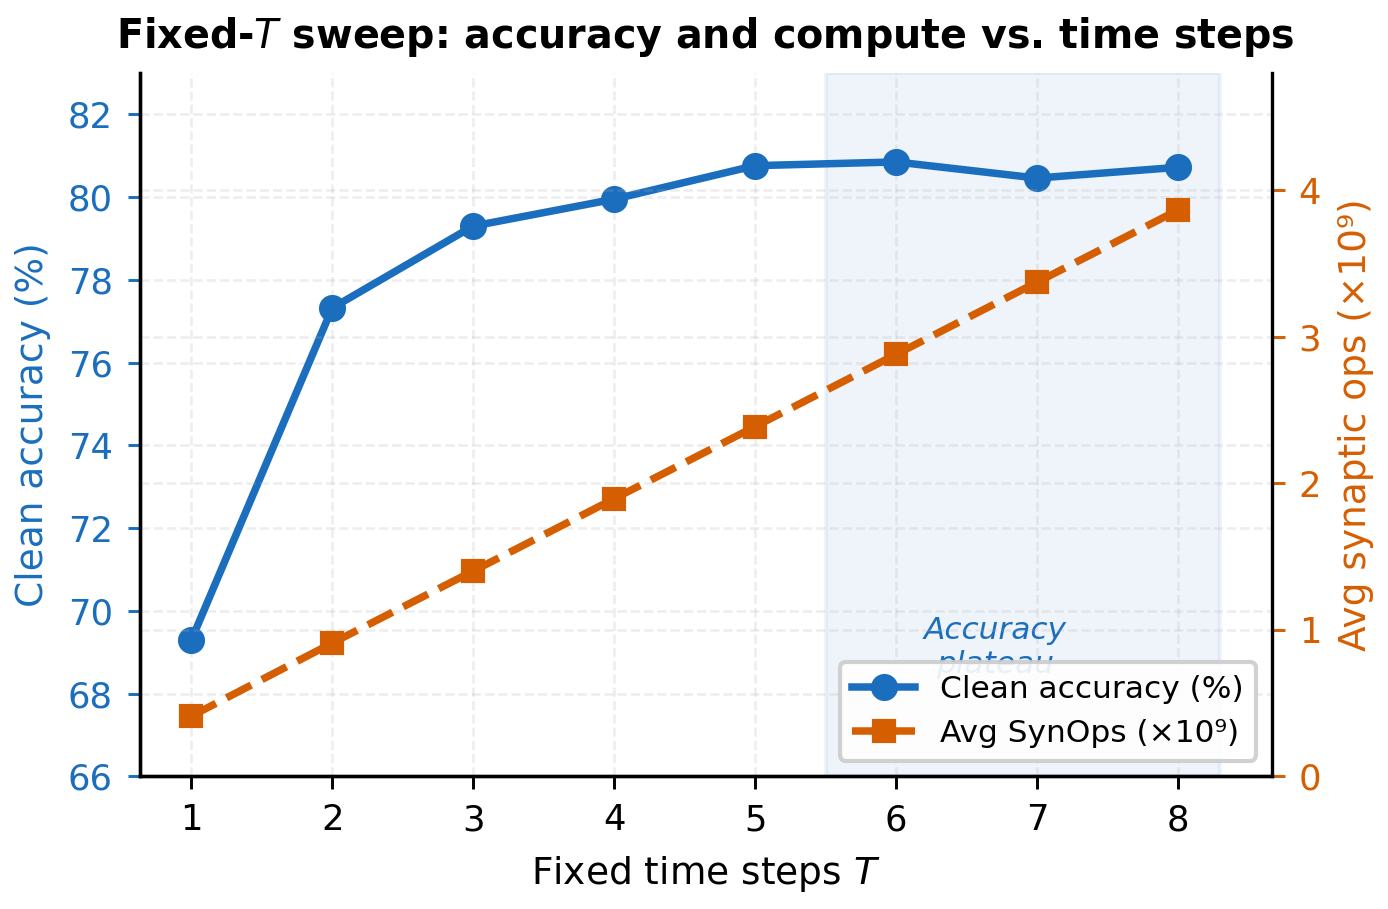
\includegraphics[width=0.92\linewidth]{figures/fig1_fixed_t_sweep.png}
\caption{Fixed-$T$ sweep on the clean test set. Accuracy rises quickly at small $T$ and then largely plateaus, while SynOps continue to increase almost linearly.}
\label{fig:fixed-sweep}
\end{figure}

\begin{table}[h]
\centering
\caption{Main clean test comparison for the completed ResNet run.}
\label{tab:main-clean}
\begin{tabular}{lccc}
\toprule
Method & Accuracy (\%) & Avg. Steps & Avg. SynOps \\
\midrule
Fixed $T=8$ & 80.72 & 8.00 & $3.864 \times 10^9$ \\
Fixed matched ($T=4$) & 79.95 & 4.00 & $1.894 \times 10^9$ \\
VT selected ($\theta=0.60$) & 80.33 & 3.78 & $1.756 \times 10^9$ \\
\bottomrule
\end{tabular}
\end{table}

Two points are especially important:
\begin{itemize}[leftmargin=1.5em]
    \item Compared with fixed $T=8$, the selected VT policy loses only \SI{0.39}{\percent} absolute clean accuracy while reducing SynOps by approximately \SI{54.57}{\percent}.
    \item Compared with the compute-matched fixed baseline ($T=4$), VT at $\theta=0.60$ gains \SI{0.38}{\percent} absolute accuracy while also using about \SI{7.32}{\percent} fewer SynOps.
\end{itemize}

This is the strongest result collected so far because it directly supports the paper's intended claim: the gain is not merely due to truncating computation; adaptive stopping is improving the clean accuracy/compute tradeoff relative to a fixed-time control. In other words, the model is not only doing ``less work'' than fixed $T=8$; it is also doing \emph{better work allocation} than a uniform fixed truncation.
Figure~\ref{fig:clean-summary} is the cleanest visual summary of this claim. The selected VT operating point $\theta=0.60$ sits in the middle of the useful trade-off region: it saves approximately \SI{54.6}{\percent} SynOps relative to fixed $T=8$ while losing only \SI{0.39}{\percent} clean accuracy, and it compares favorably to nearby fixed-$T$ controls.

\begin{figure}[t]
\centering
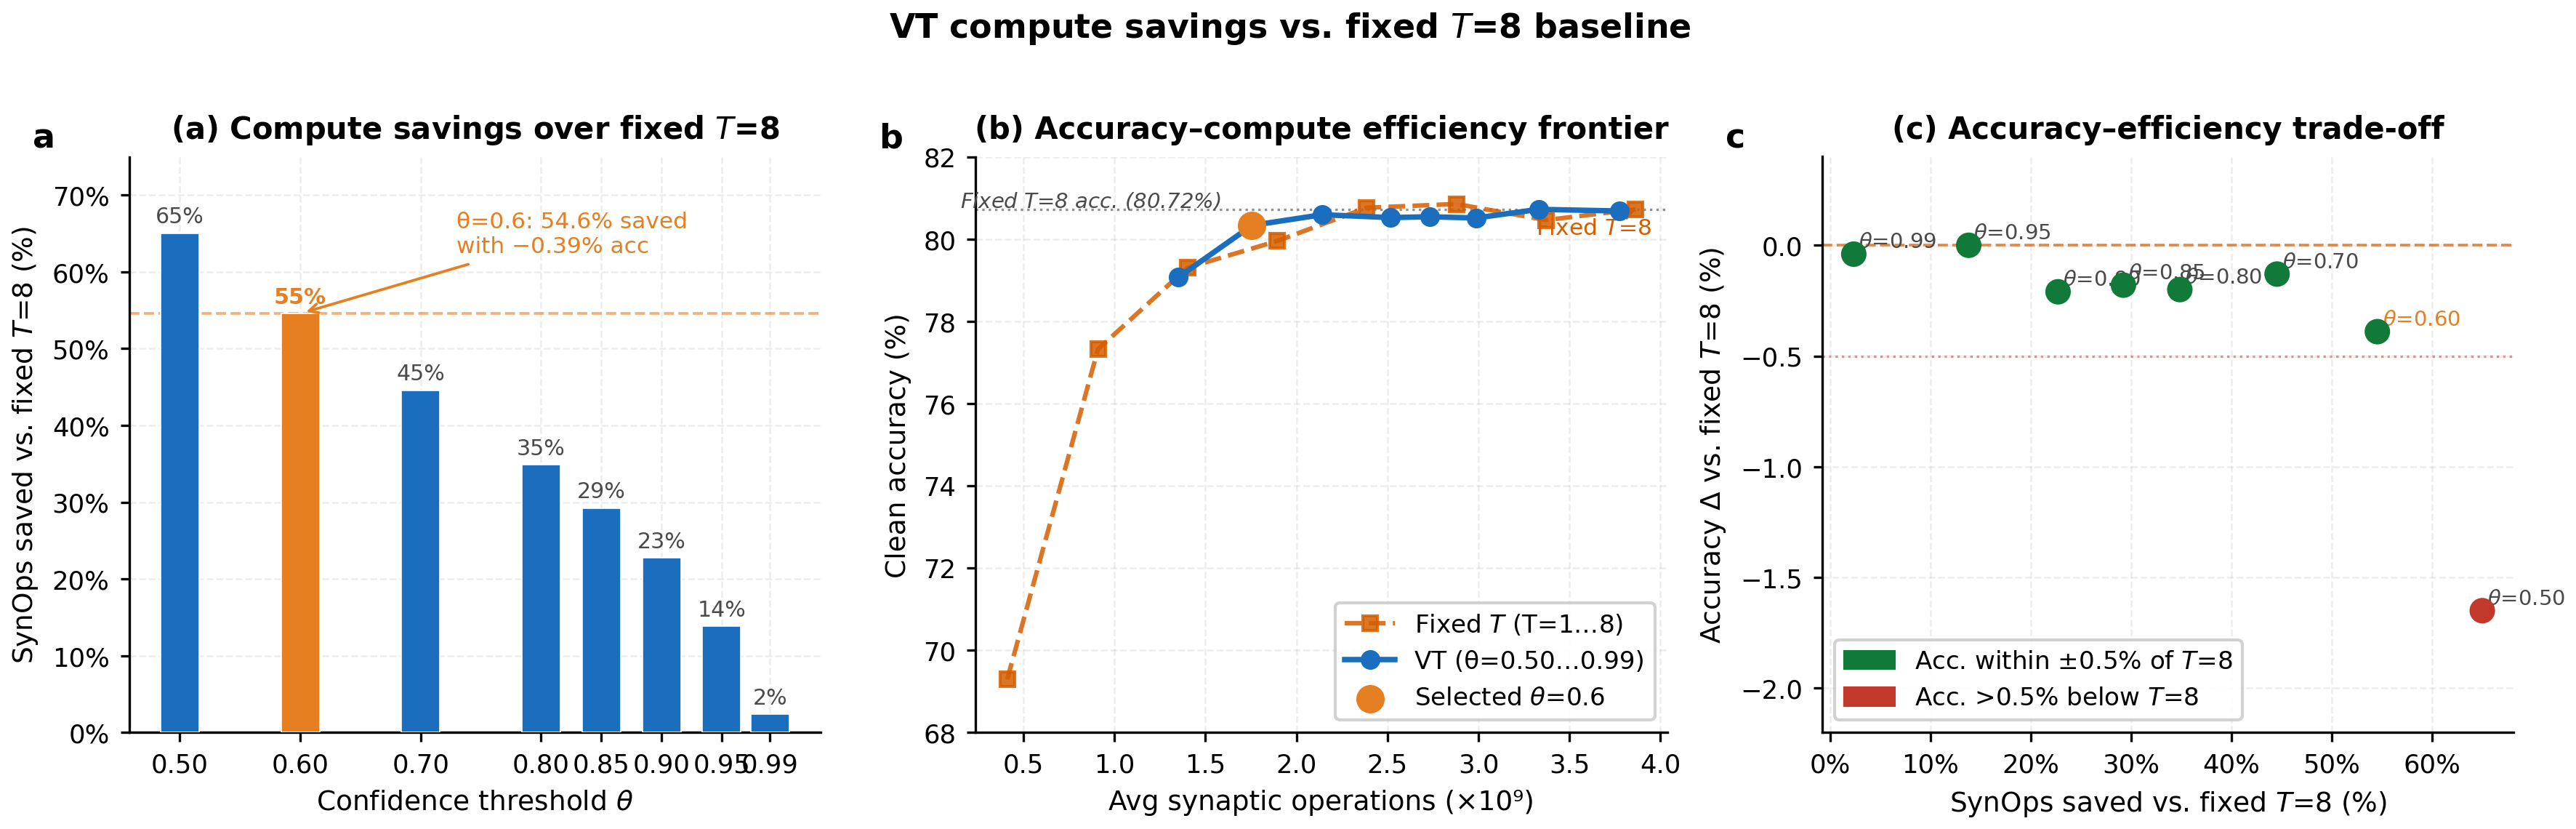
\includegraphics[width=\linewidth]{figures/fig_clean_compute_savings_vs_t8.png}
\caption{Main clean-result summary. Panel (a) shows VT compute savings relative to fixed $T=8$, panel (b) shows the clean accuracy--compute frontier, and panel (c) shows the trade-off between SynOps saved and accuracy relative to the full-horizon baseline.}
\label{fig:clean-summary}
\end{figure}

\subsection{Full VT Frontier on Test}
The full test-set VT frontier is already available. The most relevant points are summarized in Table~\ref{tab:vt-panel}.

\begin{table}[h]
\centering
\caption{Selected VT clean operating points on the test set.}
\label{tab:vt-panel}
\begin{tabular}{lccc}
\toprule
Threshold & Accuracy (\%) & Avg. Steps & Avg. SynOps \\
\midrule
$0.50$ & 79.07 & 2.94 & $1.351 \times 10^9$ \\
$0.60$ & 80.33 & 3.78 & $1.756 \times 10^9$ \\
$0.70$ & 80.59 & 4.57 & $2.142 \times 10^9$ \\
\bottomrule
\end{tabular}
\end{table}

The broader test sweep is smooth and sensible:
\begin{itemize}[leftmargin=1.5em]
    \item low thresholds save more compute but hurt clean accuracy,
    \item mid thresholds (\(0.60\)--\(0.80\)) provide the best tradeoff region,
    \item high thresholds approach the full-horizon model.
\end{itemize}

One particularly interesting observation is that $\theta=0.95$ recovers the same clean accuracy as fixed $T=8$ (\SI{80.72}{\percent}) while still using fewer SynOps ($3.330 \times 10^9$ vs. $3.864 \times 10^9$). This is not the primary operating point selected for the paper, but it suggests that the VT mechanism remains competitive even in the near-full-compute regime.
Figure~\ref{fig:vt-sweep} makes the same point from the VT side: as $\theta$ increases, the model becomes more conservative, average stopping depth rises, and accuracy approaches the full-horizon ceiling. The selected threshold $\theta=0.60$ lies near the start of the strong trade-off region rather than at the near-full-compute end.

\begin{figure}[t]
\centering
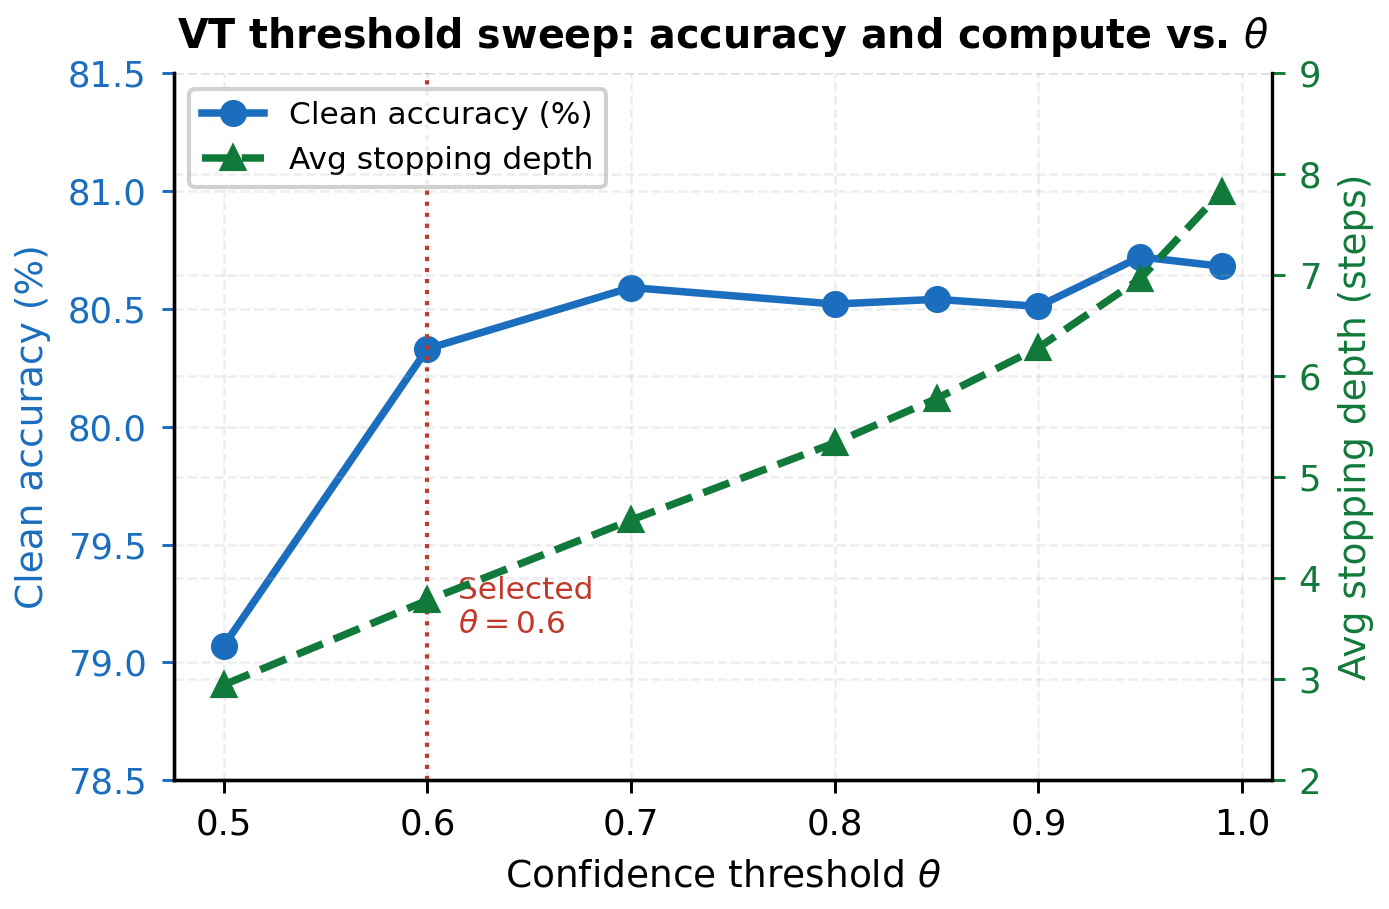
\includegraphics[width=0.92\linewidth]{figures/fig2_vt_threshold_sweep.png}
\caption{VT threshold sweep on the clean test set. Higher thresholds increase average stopping depth and push the model toward full-horizon behavior. The selected threshold $\theta=0.60$ lies in the efficient early part of the trade-off curve.}
\label{fig:vt-sweep}
\end{figure}

\subsection{Section 3: Stopping-Rule Comparison Completed}
Stopping-rule calibration and test evaluation also finished. Table~\ref{tab:stop-rules} summarizes the clean test outcomes for the current rule set.

\begin{table}[h]
\centering
\caption{Stopping-rule comparison on the test set.}
\label{tab:stop-rules}
\begin{tabular}{lccc}
\toprule
Rule & Threshold & Accuracy (\%) & Avg. SynOps \\
\midrule
Fixed $T=8$ baseline & -- & 80.72 & $3.864 \times 10^9$ \\
Max-softmax & 0.60 & 80.33 & $1.742 \times 10^9$ \\
Margin & 0.50 & 80.45 & $2.003 \times 10^9$ \\
Entropy & 0.50 & 79.68 & $1.860 \times 10^9$ \\
Temperature-softmax & 0.50 & 80.55 & $2.694 \times 10^9$ \\
Evidential surrogate & 0.50 & 77.75 & $2.162 \times 10^9$ \\
\bottomrule
\end{tabular}
\end{table}

Current interpretation:
\begin{itemize}[leftmargin=1.5em]
    \item \textbf{Max-softmax} remains the cleanest matched-compute choice.
    \item \textbf{Margin} is competitive and slightly higher in accuracy, but it uses more compute.
    \item \textbf{Temperature-softmax} attains high clean accuracy but is poorly matched in compute and therefore does not look attractive as a fair stopping-rule substitute.
    \item \textbf{Evidential surrogate} is currently weak in both accuracy and compute matching.
\end{itemize}

For the current draft, max-softmax still looks like the best main-paper rule because it aligns with the selected SynOps target while remaining simple and interpretable. The stopping-rule experiment is not asking whether one scalar confidence surrogate is philosophically ``correct.'' It is asking whether the overall VT phenomenon survives across different reasonable confidence signals. So far, the answer looks like yes, although max-softmax remains the strongest default.
Figure~\ref{fig:stop-rules} is useful here because it separates accuracy, stopping depth, and SynOps into parallel views. The figure makes clear that some alternative rules can preserve clean accuracy, but they do so at noticeably higher compute.

\begin{figure}[t]
\centering
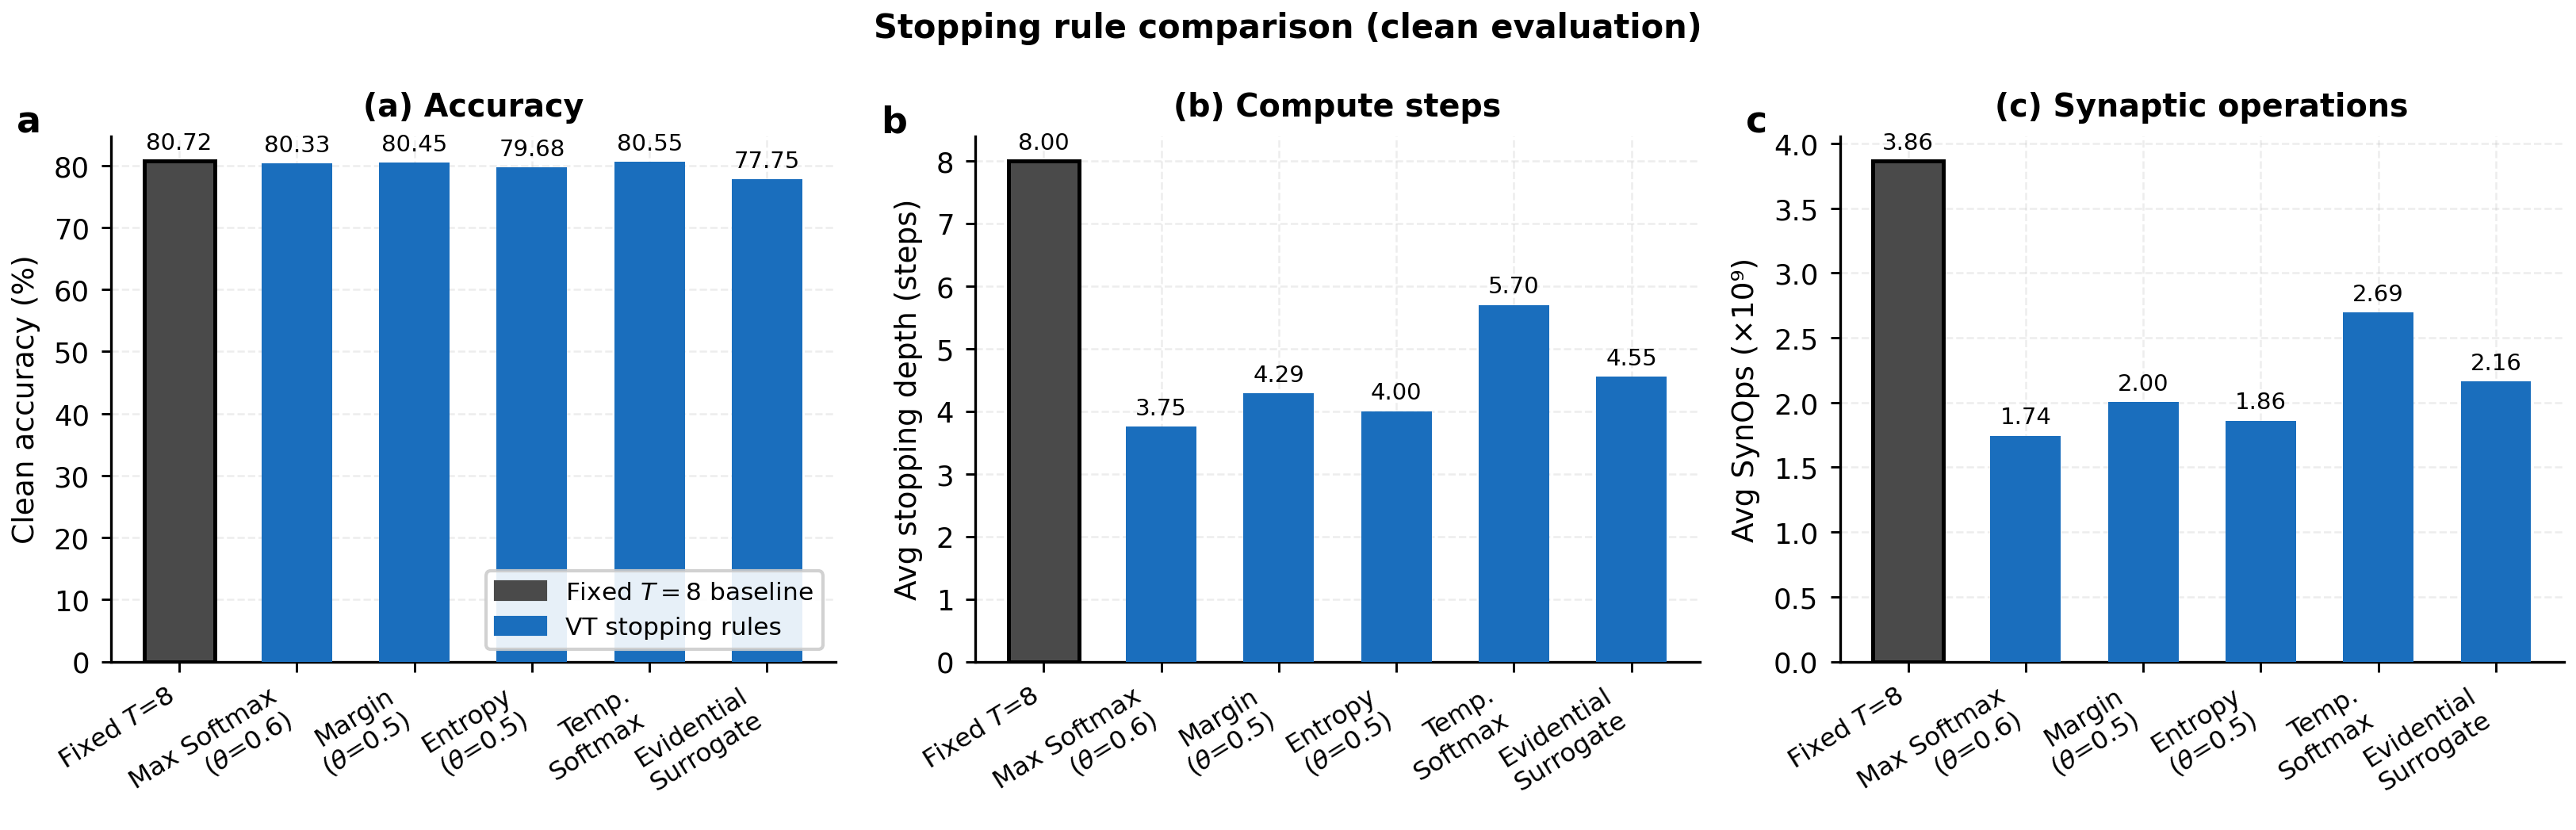
\includegraphics[width=\linewidth]{figures/fig6_stopping_rules.png}
\caption{Stopping-rule comparison on the clean test set. Max-softmax remains the most attractive default because it stays competitive in accuracy while also remaining close to the desired compute budget.}
\label{fig:stop-rules}
\end{figure}

\subsection{Section 4: Reduced Attack Study Completed on a Class-Balanced Subset}
The full stochastic attack suite proved too expensive to run end-to-end on the full CIFAR-10 test set. To keep the evaluation methodologically meaningful while remaining computationally feasible, the heavy attack block was rerun on a fixed \textbf{class-balanced 1000-sample attack subset} (100 samples per CIFAR-10 class). Clean results in Sections~1--3 still use the full test set; only the heavy attack suite uses this subset.

This is an important distinction. The attack subset is not meant to replace the full clean evaluation. It is meant to provide a tractable but still structured robustness comparison under strong adaptive attacks on the exact same backbone and selected VT thresholds.

\subsubsection{Subset Baseline Analysis}
Before interpreting the attack results, it is useful to establish the clean reference on the \emph{same} 1000-sample subset. Table~\ref{tab:attack-subset-clean} shows that the subset itself is not pathological: the fixed full-horizon baseline attains \SI{81.6}{\percent} clean accuracy, while VT remains competitive across the selected threshold panel.

\begin{table}[h]
\centering
\caption{Clean reference on the class-balanced 1000-sample attack subset.}
\label{tab:attack-subset-clean}
\begin{tabular}{lccc}
\toprule
Method & Threshold & Accuracy (\%) & Avg. Stopping Depth \\
\midrule
Fixed $T=8$ & -- & 81.6 & 8.000 \\
VT lower neighbor & 0.50 & 79.3 & 2.890 \\
VT selected & 0.60 & 81.2 & 3.667 \\
VT upper neighbor & 0.70 & 80.9 & 4.532 \\
\bottomrule
\end{tabular}
\end{table}

The selected threshold \(\theta = 0.60\) remains very close to the fixed full-horizon model even on this reduced subset, which makes it a reasonable operating point for attack comparison.

\subsubsection{Untargeted Adaptive PGD Results}
The main robustness comparison on the subset uses strong untargeted adaptive PGD with 20 steps and EOT = 8. Table~\ref{tab:attack-untargeted} shows the resulting accuracies.

\begin{table}[h]
\centering
\caption{Untargeted adaptive PGD on the class-balanced 1000-sample attack subset.}
\label{tab:attack-untargeted}
\begin{tabular}{lccc}
\toprule
Method & Threshold & Accuracy (\%) & Avg. Stopping Depth \\
\midrule
Fixed $T=8$ & -- & 39.6 & 8.000 \\
VT lower neighbor & 0.50 & 44.4 & 3.457 \\
VT selected & 0.60 & 42.0 & 4.592 \\
VT upper neighbor & 0.70 & 39.8 & 5.645 \\
\bottomrule
\end{tabular}
\end{table}

The most important observation is that VT does \emph{not} collapse under the adaptive untargeted attack. In fact, the lower and selected thresholds both outperform the fixed full-horizon baseline on this subset:
\begin{itemize}[leftmargin=1.5em]
    \item VT at \(\theta=0.50\) exceeds fixed $T=8$ by \SI{4.8}{\percent} absolute.
    \item VT at the selected threshold \(\theta=0.60\) exceeds fixed $T=8$ by \SI{2.4}{\percent} absolute.
    \item VT at \(\theta=0.70\) is essentially tied with fixed $T=8$.
\end{itemize}

This does not yet prove that VT is universally more robust than fixed full-horizon inference, because the result is on a 1000-sample attack subset rather than the entire test set. However, it is a strong indication that the clean-side VT advantage does not disappear immediately once the attack becomes adaptive and exit-aware.

\subsubsection{Wrong-Early-Exit Attack Results}
The custom \emph{wrong-early-exit} objective was designed to attack the VT mechanism more directly by encouraging confident incorrect early exits. Table~\ref{tab:attack-wrong-exit} summarizes the results.

\begin{table}[h]
\centering
\caption{Wrong-early-exit attack on the class-balanced 1000-sample attack subset.}
\label{tab:attack-wrong-exit}
\begin{tabular}{lccc}
\toprule
VT Threshold & Accuracy (\%) & Avg. Stopping Depth & Change vs Untargeted Accuracy \\
\midrule
0.50 & 42.8 & 2.715 & -1.6 \\
0.60 & 41.3 & 4.064 & -0.7 \\
0.70 & 39.8 & 5.343 & 0.0 \\
\bottomrule
\end{tabular}
\end{table}

The main interpretation is that this exit-aware objective does hurt VT somewhat, but it does not erase the effect entirely. In particular, the selected threshold drops from \SI{42.0}{\percent} under untargeted PGD to \SI{41.3}{\percent} under wrong-early-exit, which is a real degradation but not a collapse.
Figure~\ref{fig:attack-summary} summarizes the main attack-side picture. The first two panels show that attack pressure increases VT stopping depth, especially at higher thresholds, while the third panel visualizes the depth--accuracy trade-off across clean, untargeted PGD, and wrong-early-exit conditions.

\begin{figure}[t]
\centering
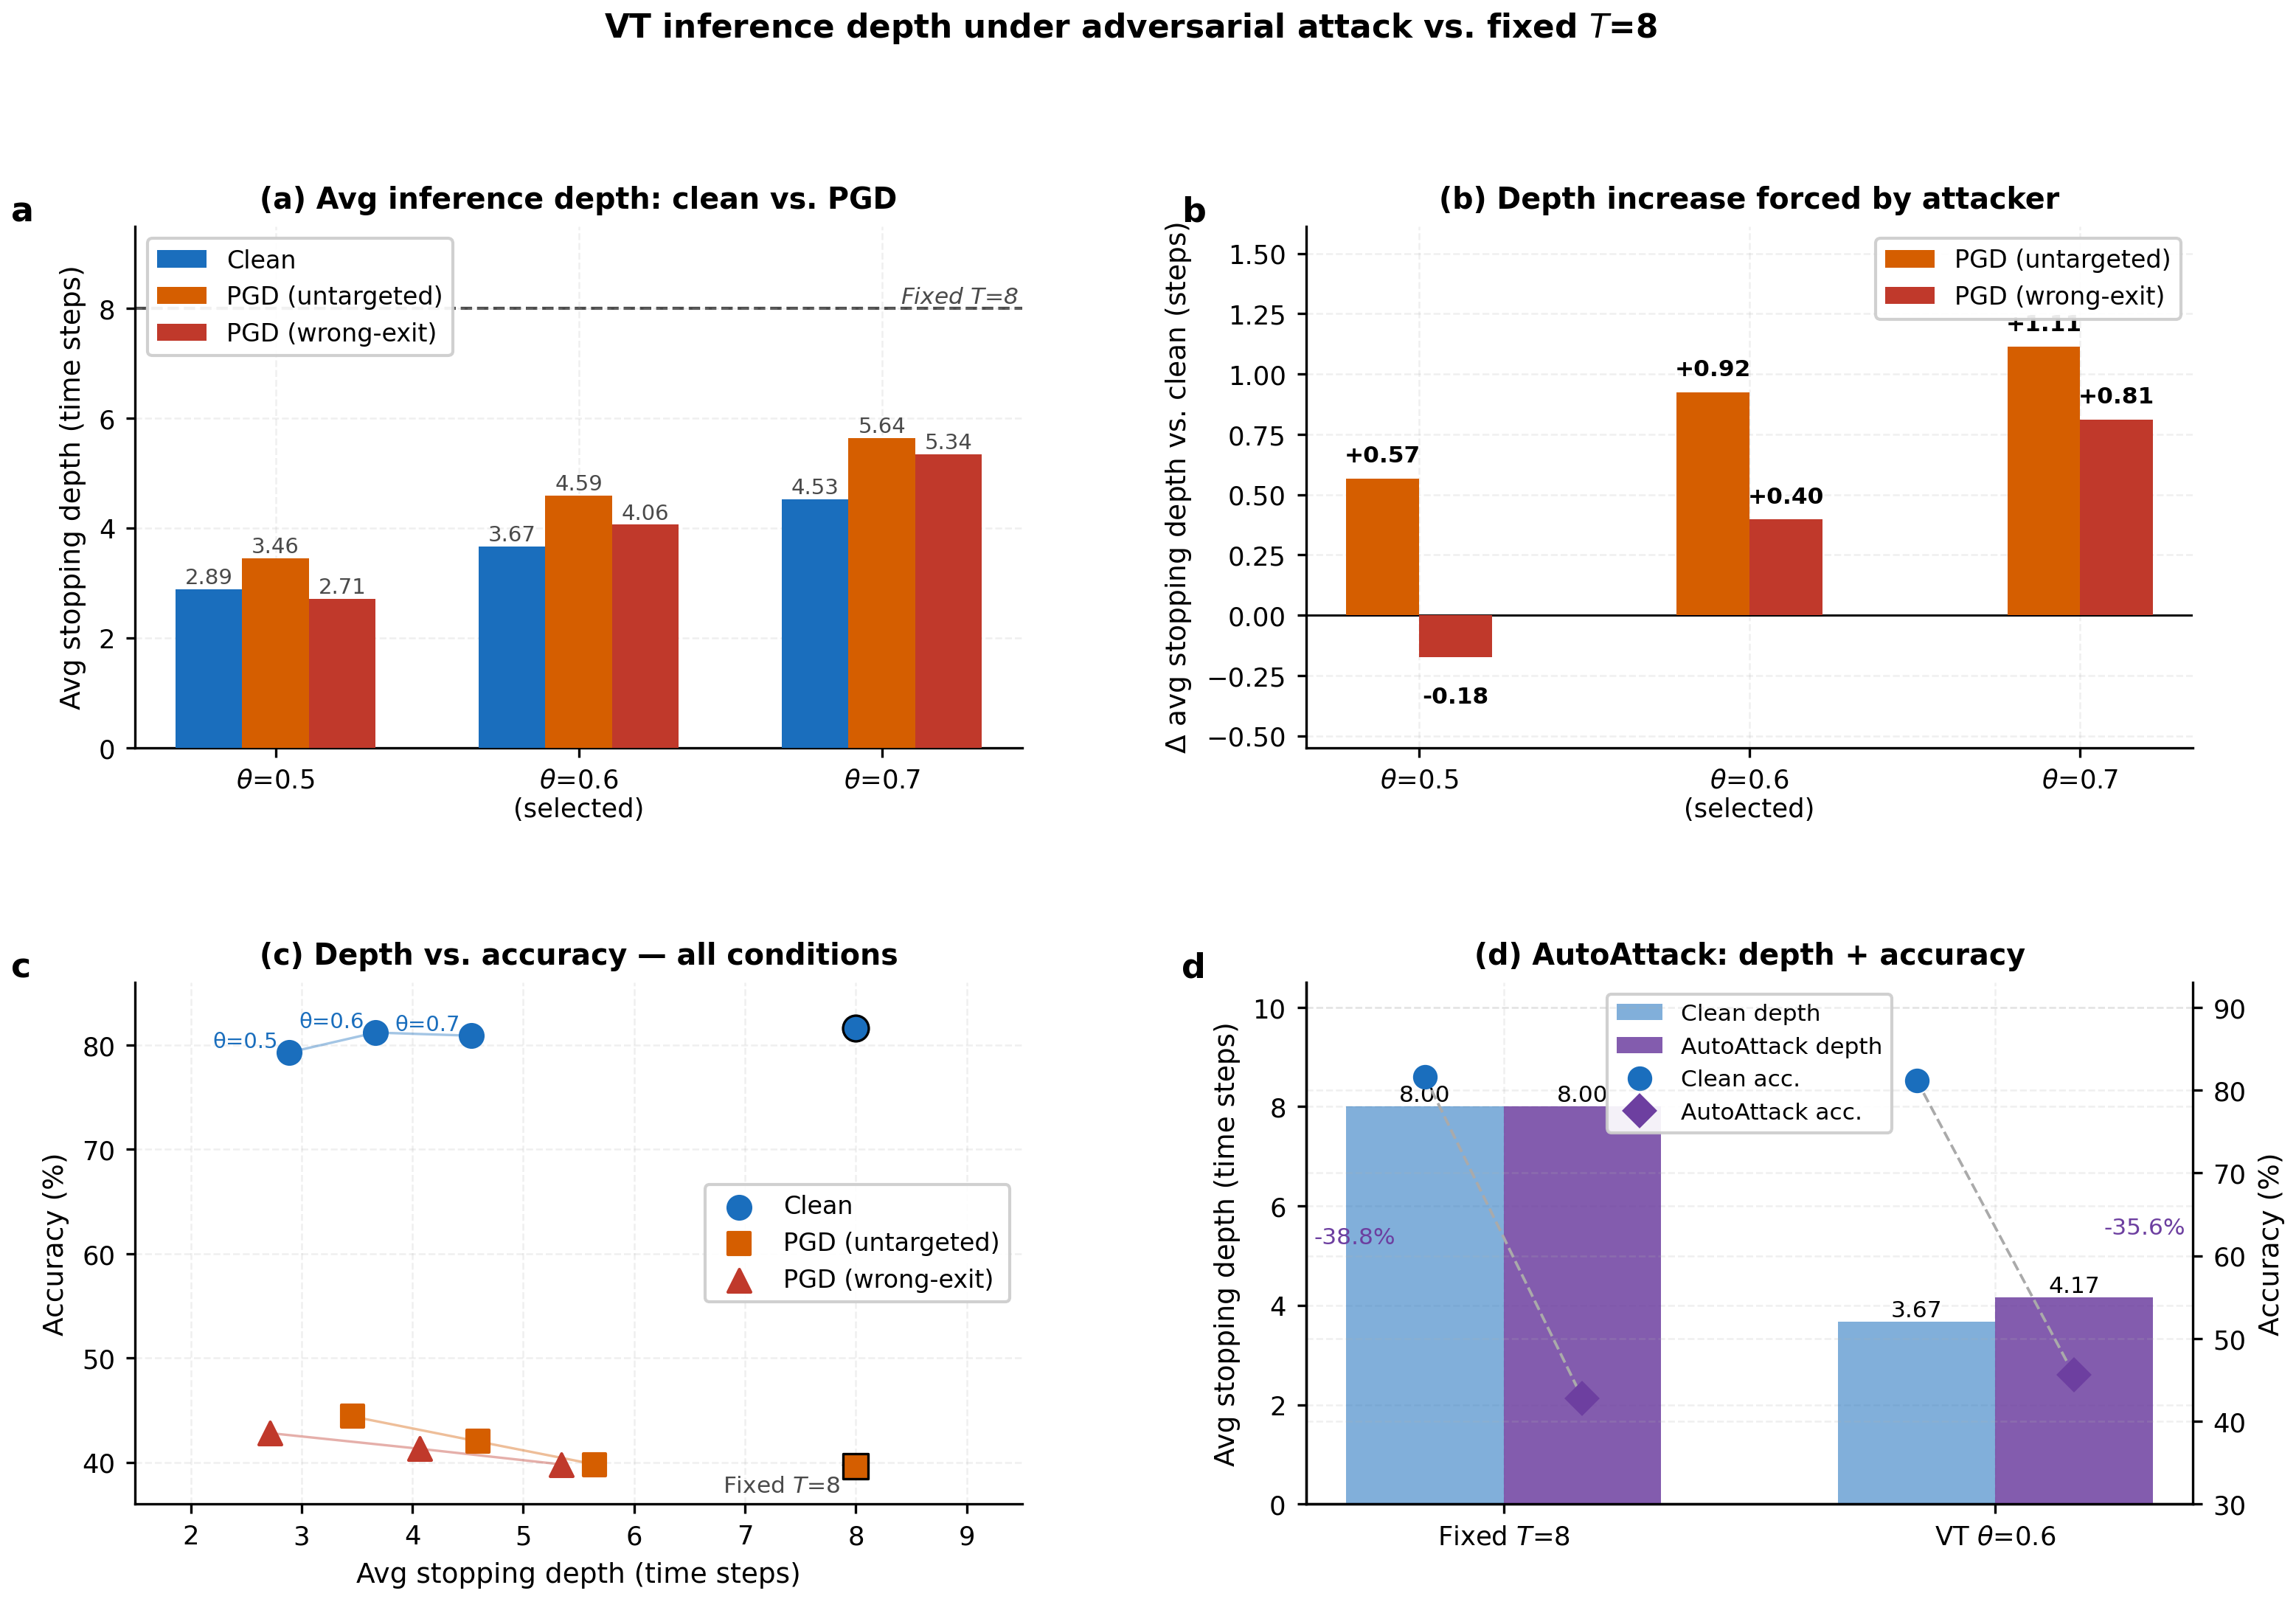
\includegraphics[width=\linewidth]{figures/fig_attack_compute_savings.png}
\caption{Attack-side summary on the reduced evaluation subsets. Panels (a)--(c) compare clean, untargeted PGD, and wrong-early-exit behavior across the selected VT threshold panel. Panel (d) adds the AutoAttack confirmation result on the smaller balanced subset.}
\label{fig:attack-summary}
\end{figure}

\subsubsection{Compute-Overuse Results}
The custom \emph{compute-overuse} objective is not a standard robustness attack in the usual misclassification sense. Its purpose is to test whether a bounded perturbation can force the VT mechanism to consume \emph{more computation} while largely preserving the predicted label. Therefore the main quantity of interest is not attacked accuracy but the increase in stopping depth relative to clean evaluation on the same subset.

Table~\ref{tab:attack-compute-overuse} shows the clean-versus-attacked depth comparison.

\begin{table}[h]
\centering
\caption{Compute-overuse attack on the class-balanced 1000-sample attack subset.}
\label{tab:attack-compute-overuse}
\begin{tabular}{lcccc}
\toprule
VT Threshold & Clean Acc. (\%) & Attacked Acc. (\%) & Clean Depth & Depth Increase \\
\midrule
0.50 & 79.3 & 94.9 & 2.890 & +0.207 \\
0.60 & 81.2 & 97.2 & 3.667 & +0.629 \\
0.70 & 80.9 & 97.3 & 4.532 & +1.154 \\
\bottomrule
\end{tabular}
\end{table}

The attacked accuracies are higher than the clean accuracies because this objective explicitly rewards preserving the label while increasing computation. Therefore these numbers should not be interpreted as ``robust accuracy'' in the normal sense. The relevant result is that a bounded perturbation can increase stopping depth by a meaningful amount:
\begin{itemize}[leftmargin=1.5em]
    \item \(\theta=0.50\): +0.207 average steps,
    \item \(\theta=0.60\): +0.629 average steps,
    \item \(\theta=0.70\): +1.154 average steps.
\end{itemize}

This gives concrete support for the paper's proposed latency/energy denial-of-service angle. The effect becomes stronger as the threshold becomes more conservative, which is intuitively reasonable: when the clean operating point already sits closer to the full horizon, there is more room for an attacker to push it further toward maximum compute.
Figure~\ref{fig:compute-overuse} makes this especially clear. The left panel shows why compute-overuse accuracy should not be read as ordinary robust accuracy: the attack objective explicitly rewards label preservation. The right panel is the real result, namely that the attacker can force deeper inference, and that the effect becomes larger as the VT threshold becomes more conservative.

\begin{figure}[t]
\centering
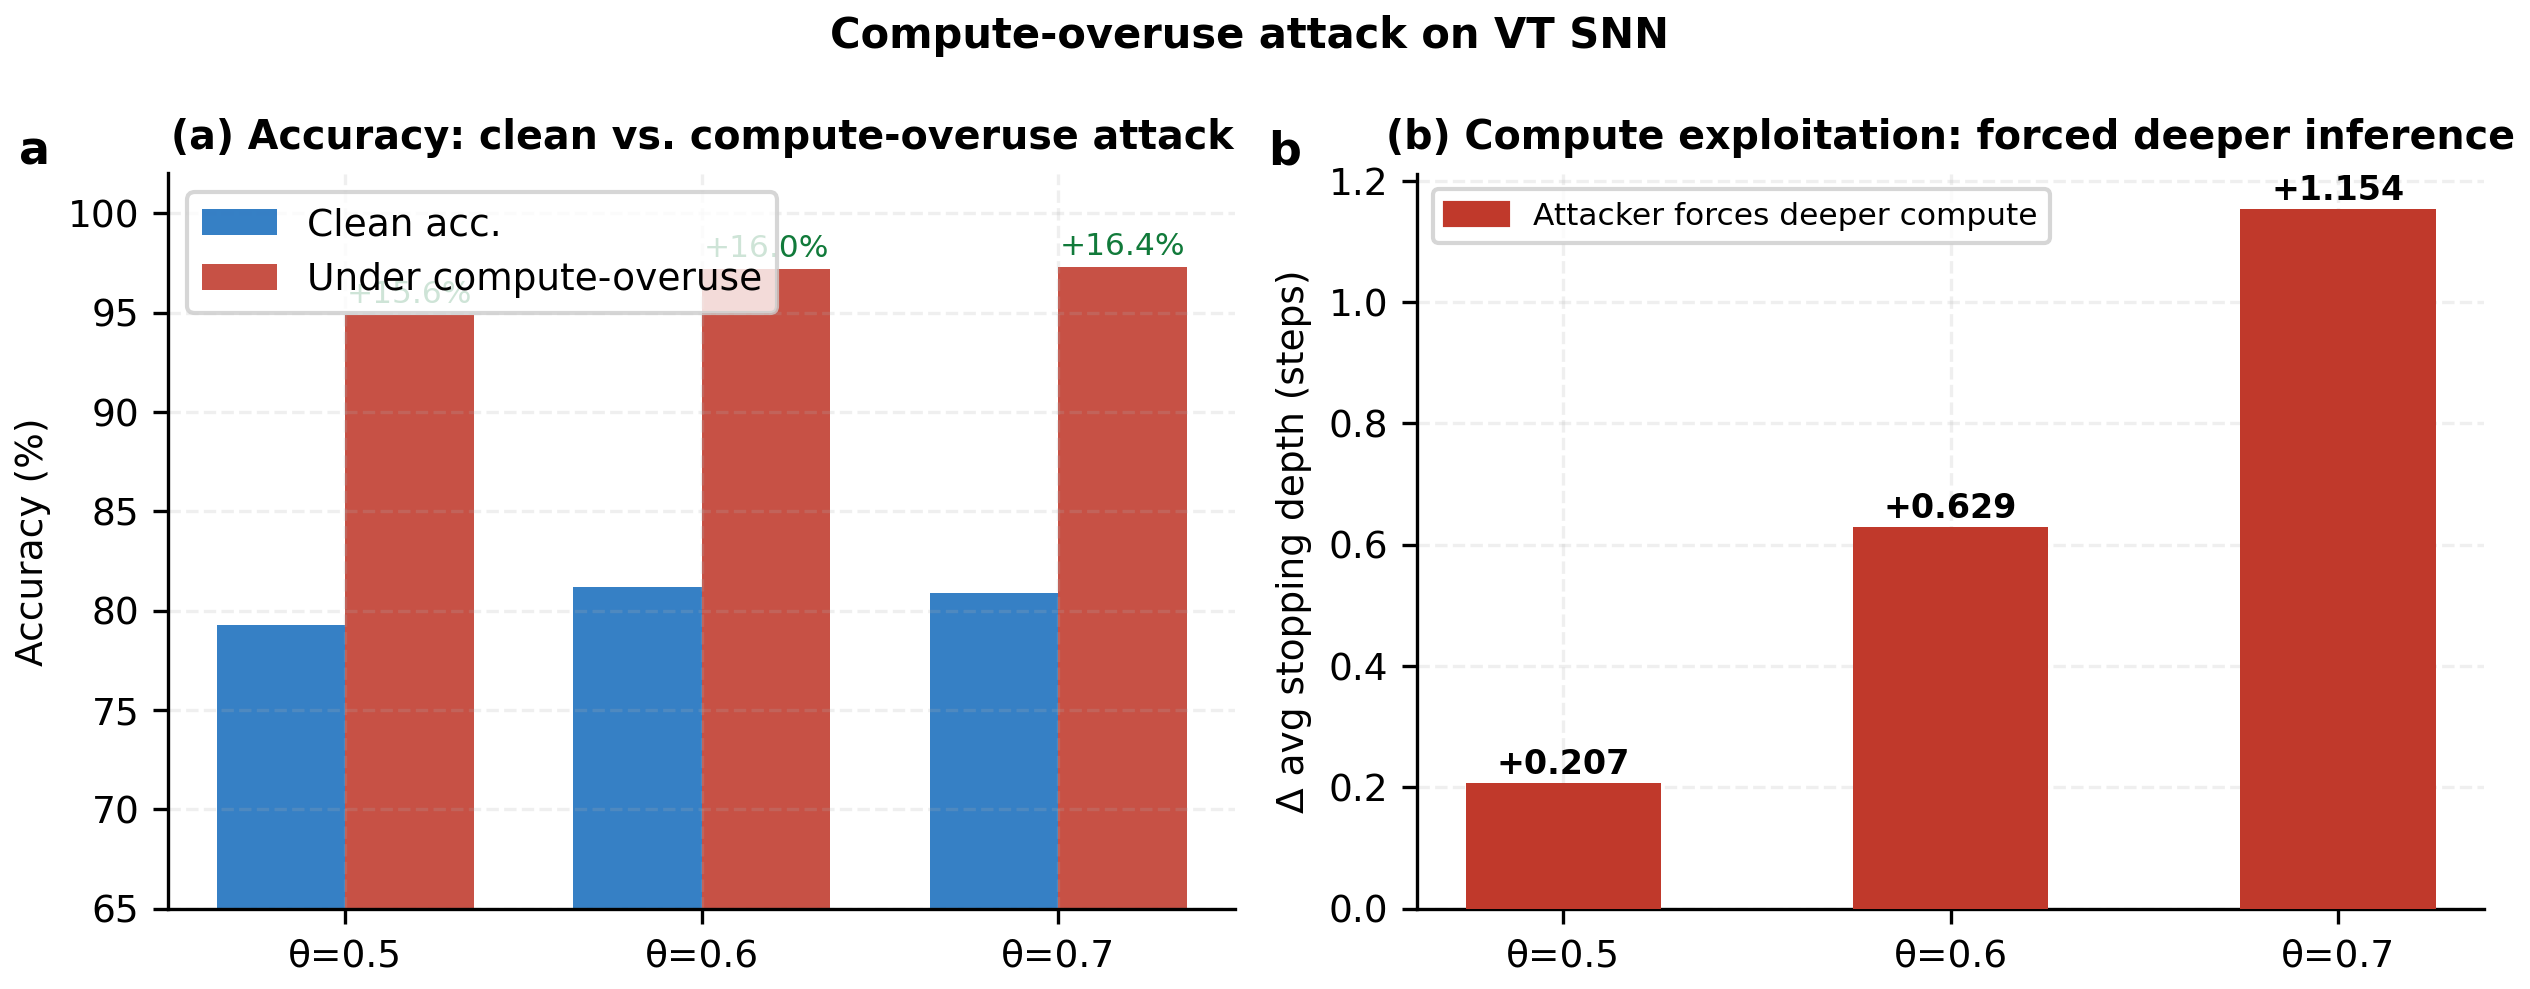
\includegraphics[width=\linewidth]{figures/fig5_compute_overuse.png}
\caption{Compute-overuse attack on the 1000-sample balanced subset. The relevant effect is not misclassification but increased stopping depth under bounded perturbation.}
\label{fig:compute-overuse}
\end{figure}

\subsubsection{AutoAttack Confirmation on a Smaller Balanced Subset}
A smaller but stronger confirmation experiment was also completed with vectorized AutoAttack on a fixed balanced 250-sample subset at EOT = 4. This run is smaller than the 1000-sample PGD subset and therefore should not be treated as directly interchangeable with it, but it is still useful as a stress test because AutoAttack is substantially stronger and harder to tune accidentally.

On this 250-sample subset:
\begin{itemize}[leftmargin=1.5em]
    \item fixed $T=8$ attains \SI{42.8}{\percent} accuracy,
    \item VT at the selected threshold $\theta=0.60$ attains \SI{45.6}{\percent} accuracy.
\end{itemize}

Therefore VT retains a \SI{2.8}{\percent} absolute advantage over the fixed full-horizon baseline even under this stronger confirmation run. This does not replace a full-scale stochastic AutoAttack study, but it is consistent with the PGD subset results and therefore strengthens the overall claim that the VT advantage is not merely a weak-attack artifact.

\section{Work Still Remaining}
The clean evaluation story is substantially complete for the first ResNet model, and the reduced attack study now provides an initial robustness picture. However, the most important missing components are still significant.

\subsection{Paused Due to Runtime / Compute Constraints}
The following components are implemented in the codebase but not completed for this ResNet run because Kaggle is too slow and too fragile for the heaviest stages:
\begin{itemize}[leftmargin=1.5em]
    \item \textbf{Full-scale Section 4:} broader attack coverage beyond the reduced 1000-sample subset study,
    \item \textbf{Stochastic AutoAttack at larger scale:} still computationally prohibitive with full-trace EOT, even though a smaller 250-sample confirmation run has now been completed,
    \item \textbf{Section 5:} ablation matrix,
    \item optional heavier evaluations such as multi-seed exact VT and large attack sweeps.
\end{itemize}

The bottleneck is not plain GPU throughput alone. The attack path combines time-unrolled gradients, exit-aware objectives, stochastic EOT, and VT inference, which creates severe runtime and memory pressure even on strong hardware. For this reason, the current reduced attack study uses batched-proxy accounting rather than sample-exact SynOps measurement inside the attack loop.

\subsection{Still Needed Before Paper Writing}
Before turning this into a submission-quality paper, the following work remains:
\begin{enumerate}[leftmargin=1.5em]
    \item Decide on the final attack protocol:
    \begin{itemize}[leftmargin=1.5em]
        \item full-test adaptive PGD/EOT as the primary stochastic robustness benchmark,
        \item subset-based AutoAttack as a confirmation experiment if full stochastic AutoAttack remains infeasible,
        \item possibly one stronger overnight AutoAttack subset run with reduced sample count rather than chasing full-test coverage.
    \end{itemize}
    \item Run the minimal ablation matrix:
    \begin{itemize}[leftmargin=1.5em]
        \item baseline robust SNN,
        \item baseline + VT,
        \item baseline + VT + dynamic sigma,
        \item baseline + VT + Parseval,
        \item full model.
    \end{itemize}
    \item Repeat the completed clean pipeline for VGG and WRN to verify that the effect is not specific to one backbone.
    \item Run at least one small multi-seed study for the main backbone.
    \item If time allows, add one more dataset after the core CIFAR-10 result is stabilized.
\end{enumerate}

\section{Current Takeaway}
The ResNet evidence is now stronger than a clean-only story. The project currently supports the following intermediate conclusion:
\begin{quote}
Variable-timing inference appears to improve the clean accuracy/compute frontier relative to matched fixed-time baselines in an adversarially trained SNN, and that advantage does not disappear immediately under strong adaptive attacks on reduced but structured attack subsets.
\end{quote}

This is not yet the final paper claim because the robustness side is still incomplete, especially for larger-scale AutoAttack-style confirmation and for other backbones. However, the completed data already justify continuing the project. The clean-side evidence is coherent, the matched-control result is favorable to VT, the stopping-rule study suggests that max-softmax remains a reasonable default, the reduced 1000-sample PGD study indicates that VT retains a meaningful advantage under strong untargeted adaptive attacks, and the 250-sample EOT=4 AutoAttack run points in the same direction.

\section{Immediate Next Step}
The best next use of effort is still not writing the paper yet. The best next step is to consolidate the reduced attack protocol into a final reproducible form, then repeat the clean pipeline and the reduced attack study for VGG and WRN. In parallel, deterministic baselines should be evaluated so the final claim can distinguish between stochastic-specific behavior and more general VT behavior. Once those runs are available, the paper can be written around a much more defensible experimental core.

\end{document}
